\chapter{FuzzTesting e Sanitization}

Il \textbf{fuzzing} o \textbf{fuzz testing} è una tecnica di test automatizzata
del software che consiste nel fornire dati non validi, inaspettati o comunque casuali
come input ad un programma. In questo modo mettiamo in crisi il programma,
vediamo come reagisce alle varie possibilità e riusciamo a capire se ci sono bug o no.
Consiste quindi in una strategia per trovare problemi di affidabilità (reliability);
alcuni di essi possono in realtà rappresentare vulnerabilità.
Qualsiasi interfaccia di applicazione (per esempio, rete, input di file, riga di comando,
modulo Web e così via) può essere sottoposta a fuzz-test.
Gli obiettivi del fuzzing possono variare a seconda del tipo di interfaccia che si sta testando.

\begin{figure}[H]
    \centering
    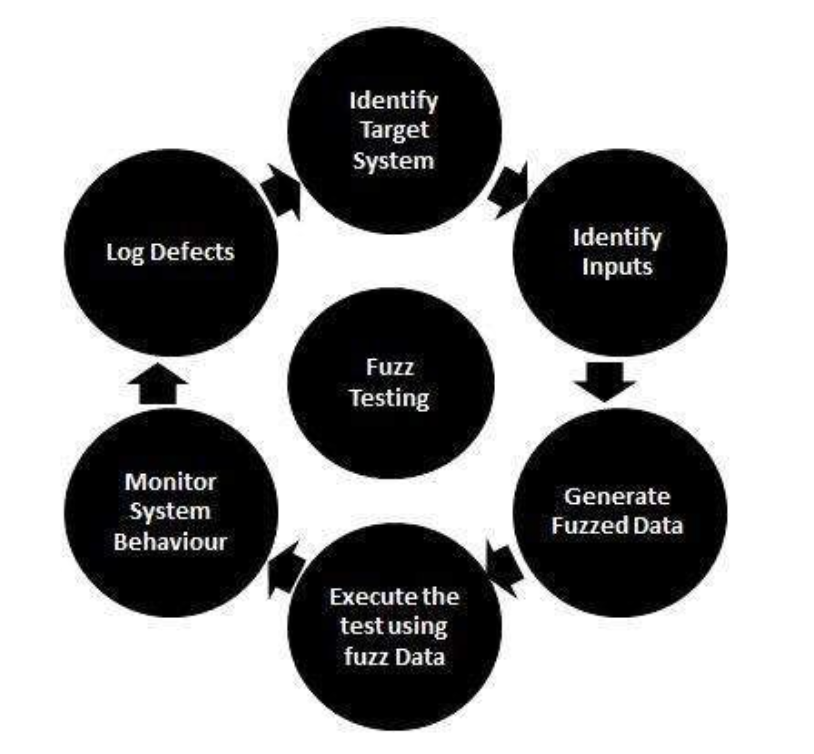
\includegraphics[width=8cm, keepaspectratio]{capitoli/secure_coding/img/cap_7/lifecycle.png}
    \caption{Lifecycle del fuzz testing.}
\end{figure}

Anche in questo caso esistono tools dinamici di sicurezza.
Si dividono in:

\begin{itemize}
    \item \textbf{Black-box} fuzzing: non presuppongono niente riguardo il programma,
          semplicemente eseguono i propri compiti. Modificano a caso ("fuzz") l'input ben formato
          cioè scritto bene.
    \item \textbf{White-box} fuzzing: hanno la possibilità di vedere il codice ed agire di
          conseguenza sull'input.
\end{itemize}

\section{White-box vs Black-box}

\paragraph{Black-box fuzzing}: consiste nell'invio di dati malformati senza verifica
effettiva di quali percorsi di codice sono stati colpiti e quali no; non vede il codice.
È più semplice da scrivere e da utilizzare, ma meno efficace.

\paragraph{White-box fuzzing}: consiste nell'invio di malformati con verifica.
È a conoscenza dei vari percorsi che fanno le informazioni nel programma ed è in grado di
generare dati più ottimizzati, al fine di tirare fuori i comportamenti inaspettati.
Attraversa quindi tutte le validazioni dei dati nel codice testato.
Risulta però essere più difficili da scrivere di un Black-box fuzzer.\\

Il black-box ha una \textit{path coverage} del codice inferiore rispetto a tecniche più
sofisticate come il fuzzing automatico delle white-box
(che viene anche detto “fuzzing intelligente”).
Si raccomanda generalmente l'utilizzo di un mix di metodologie per massimizzare
l'efficacia della scoperta della vulnerabilità.

\section{Tools}

Di seguito alcuni strumenti per il fuzz-testing del codice.

\paragraph{CERT Basic Fuzzing Framework,} in breve BFF, è uno strumento di test
black-box del software che trova difetti nelle applicazioni che girano su piattaforme Windows,
Linux e macOs. BFF raccoglie automaticamente i casi di test che causano il crash del software.

\paragraph{LibFuzzer} è uno strumento per effettuare fuzz-testing di librerie o programmi.
Viene selezionato uno specifico punto di ingresso (la funzione a cui passare gli input)
chiamata \textit{target function} per poi tenere traccia di quali aree del codice
vengono raggiunte. Vengono anche generate delle mutazioni sul
\textit{corpus} di dati in ingresso al fine di massimizzare la copertura del codice.
I fuzzer coverage-guided come libFuzzer sono \textbf{black-box} e si basano su un
corpus di input,
campione per il codice in prova, che è uguale per tutti.
Questo corpus dovrebbe idealmente essere riempito con una collezione variegata di input
validi e non validi per il codice in prova.
Il fuzzer genera mutation casuali basate sugli ingressi del campione nel corpus corrente.
Se una mutation fa scattare l'esecuzione di un path non coperto in precedenza,
allora quella mutazione viene salvata nel corpus per le future variazioni.

\paragraph{Address sanitizer} è un rilevatore di errori di memoria veloce.
È un fuzz tester focalizzato sugli indirizzi; vede cosa succede se vengono passati degli
strani indirizzi di memoria.
È costituito da un modulo del compilatore di C++ e da una libreria di run-time.
Lo strumento è in grado di rilevare i seguenti tipi di bug:

\begin{itemize}
    \item Accessi Out-of-bounds a heap, stack and globals;
    \item Use-after-free;
    \item Use-after-return;
    \item Use-after-scope;
    \item Double-free, invalid free;
    \item Memory leaks (sperimentale).
\end{itemize}

\paragraph{Undefined Behavior Sanitizer,} in breve UBSan, è un altro fuzz tester per Clang.
È un rivelatore di comportamento rapido e indefinito.
UBSan modifica il programma al momento della compilazione per rilevare, ad esempio,
vari tipi di comportamenti indefiniti durante l'esecuzione del programma:

\begin{itemize}
    \item Overflow di Signed integer;
    \item Conversione in, da, o tra tipi a virgola mobile, che causerebbero l'overflow della
          destinazione;
    \item Utilizzo di un puntatore disallineato o nullo.
\end{itemize}